% !Mode:: "TeX:UTF-8"

% 定义编译方式 dvipdfmx 或者 pdflatex,默认为 dvipdfmx
% 方式编译,如果需要修改,只需改变花括号中的内容即可。
\def\usewhat{pdflatex}

% book作为文档类
% 插入空白页可以设置openright
\documentclass[12pt,openany,oneside]{book}

% 定义本文所使用宏包
% !Mode:: "TeX:UTF-8"

% 原作者信息Original Authors:
% 张井   Jing Zhang: prayever@gmail.com     天津大学2010级管理与经济学部信息管理与信息系统专业硕士生
% 余蓝涛 Lantao Yu: lantaoyu1991@gmail.com  天津大学2008级精密仪器与光电子工程学院测控技术与仪器专业本科生

% 中大移植版by林海涛&徐浩晖

%%%%%%%%%% Package %%%%%%%%%%%%

% 支持插图处理
\usepackage{graphicx}
\usepackage[a4paper,text={146.4true mm,239.2 true mm},top= 26.2true mm,left=31.8 true mm,head=6true mm,headsep=6.5true mm,foot=16.5true mm]{geometry}

% 支持版面尺寸设置
% 支持国际标准单位
\usepackage[squaren]{SIunits}               

\usepackage{titlesec}                       % 控制标题的宏包
\usepackage{titletoc}                       % 控制目录的宏包
\usepackage{fancyhdr}                       % fancyhdr宏包 支持页眉和页脚的相关定义
\usepackage[UTF8]{ctex}                     % 支持中文显示
\usepackage{CJKpunct}                       % 精细调整中文的标点符号
\usepackage{color}                          % 支持彩色
\usepackage{amsmath}                        % AMSLaTeX宏包 用来排出更加漂亮的公式
\usepackage{amssymb}                        % 数学符号生成命令
\usepackage[below]{placeins}    %允许上一个section的浮动图形出现在下一个section的开始部分,还提供\FloatBarrier命令,使所有未处理的浮动图形立即被处理
\usepackage{multirow}                       % 使用Multirow宏包,使得表格可以合并多个row格
\usepackage{booktabs}                       % 表格,横的粗线;\specialrule{1pt}{0pt}{0pt}
\usepackage{longtable}                      % 支持跨页的表格。
\usepackage{tabularx}                       % 自动设置表格的列宽
\usepackage{subfigure}                      % 支持子图 %centerlast 设置最后一行是否居中
\usepackage[subfigure]{ccaption}            % 支持子图的中文标题
\usepackage[sort&compress,numbers]{natbib}  % 支持引用缩写的宏包
\usepackage{enumitem}                       % 使用enumitem宏包,改变列表项的格式
\usepackage{calc}                           % 长度可以用+ - * / 进行计算
\usepackage{txfonts}                        % 字体宏包
\usepackage{bm}                             % 处理数学公式中的黑斜体的宏包
\usepackage[amsmath,thmmarks,hyperref]{ntheorem}  % 定理类环境宏包,其中 amsmath 选项用来兼容 AMS LaTeX 的宏包
\usepackage{CJKnumb}                        % 提供将阿拉伯数字转换成中文数字的命令
\usepackage{indentfirst}                    % 首行缩进宏包
\usepackage{CJKutf8}                        % 用在UTF8编码环境下,它可以自动调用CJK,同时针对UTF8编码作了设置
%\usepackage{hypbmsec}                      % 用来控制书签中标题显示内容
\newcommand{\tabincell}[2]{\begin{tabular}{@{}#1@{}}#2\end{tabular}}
\usepackage{xcolor}
%支持代码环境
\usepackage{listings}
\lstset{numbers=left,
language=[ANSI]{C},
numberstyle=\tiny,
extendedchars=false,
showstringspaces=false,
breakatwhitespace=false,
breaklines=true,
captionpos=b,
keywordstyle=\color{blue!70},
commentstyle=\color{red!50!green!50!blue!50},
frame=shadowbox,
rulesepcolor=\color{red!20!green!20!blue!20}
}
%支持算法环境
\usepackage[boxed,ruled,lined]{algorithm2e}
\usepackage{algorithmic}

\usepackage{array}
\newcommand{\PreserveBackslash}[1]{\let\temp=\\#1\let\\=\temp}
\newcolumntype{C}[1]{>{\PreserveBackslash\centering}p{#1}}
\newcolumntype{R}[1]{>{\PreserveBackslash\raggedleft}p{#1}}
\newcolumntype{L}[1]{>{\PreserveBackslash\raggedright}p{#1}}

% 生成有书签的 pdf 及其生成方式。通常可以在 tjumain.tex 文件的第一行选择 pdflatex 或者是 dvipdfmx 编译手段。如果选择前者,则使用 pdflatex + pdflatex 编译; 如果选择后者,在编译的时候选择 latex + bibtex + latex + latex 编译。出现混淆的时候,系统会报错。
% 如果您的pdf制作中文书签有乱码使用如下命令,就可以解决了
\def\atemp{dvipdfmx}\ifx\atemp\usewhat
\usepackage[dvipdfmx,unicode,               % dvipdfmx 编译, 加入了中文复制,粘贴支持引擎。
            pdfstartview=FitH,
            bookmarksnumbered=true,
            bookmarksopen=true,
            colorlinks=false,
            pdfborder={0 0 1},
            citecolor=blue,
            linkcolor=red,
            anchorcolor=green,
            urlcolor=blue,
            breaklinks=true
            ]{hyperref}
\fi

\def\atemp{pdflatex}\ifx\atemp\usewhat
\usepackage{cmap}                           % pdflatex 编译时,可以生成可复制、粘贴的中文 PDF 文档, 缺点是在Windows上显示时效果不大好,字体发虚
\usepackage[pdftex,unicode,
            %CJKbookmarks=true,
            bookmarksnumbered=true,
            bookmarksopen=true,				
            hidelinks
%            colorlinks=true,		% original false
%            pdfborder={0 0 1},
%            citecolor=black,		% original blue
%            linkcolor=black,		% original red
%            anchorcolor=black,		% original green
%            urlcolor=blue,
%            breaklinks=false		% original true
            ]{hyperref}
\fi

% 新增for url
\usepackage{url}


% 定义所有的.eps/.pdf图片文件在figures子目录下
\graphicspath{{figures/}}

\begin{document}

% 开始中文字体使用
\begin{CJK*}{UTF8}{song}

% 完成对论文各个部分格式的设置
% !Mode:: "TeX:UTF-8"

%%%%%%%%%%%%%%%%% Fonts Definition and Basics %%%%%%%%%%%%%%%%%
\newcommand{\song}{\CJKfamily{song}}    % 宋体
\newcommand{\fs}{\CJKfamily{fs}}        % 仿宋体
\newcommand{\kai}{\CJKfamily{kai}}      % 楷体
\newcommand{\hei}{\CJKfamily{hei}}      % 黑体
\newcommand{\li}{\CJKfamily{li}}        % 隶书
\newcommand{\chuhao}{\fontsize{28pt}{28pt}\selectfont}       % 初号, 单倍行距
\newcommand{\yihao}{\fontsize{26pt}{26pt}\selectfont}       % 一号, 单倍行距
\newcommand{\xiaoyi}{\fontsize{24pt}{24pt}\selectfont}      % 小一, 单倍行距
\newcommand{\erhao}{\fontsize{22pt}{1.25\baselineskip}\selectfont}       % 二号, 1.25倍行距
\newcommand{\xiaoer}{\fontsize{18pt}{18pt}\selectfont}      % 小二, 单倍行距
\newcommand{\sanhao}{\fontsize{16pt}{16pt}\selectfont}      % 三号, 单倍行距
\newcommand{\xiaosan}{\fontsize{15pt}{15pt}\selectfont}     % 小三, 单倍行距
\newcommand{\sihao}{\fontsize{14pt}{14pt}\selectfont}       % 四号, 单倍行距
\newcommand{\xiaosi}{\fontsize{12pt}{12pt}\selectfont}      % 小四, 单倍行距
\newcommand{\wuhao}{\fontsize{10.5pt}{10.5pt}\selectfont}   % 五号, 单倍行距
\newcommand{\xiaowu}{\fontsize{9pt}{9pt}\selectfont}        % 小五, 单倍行距

% 重新定义了波浪符~的意义
\CJKtilde

% 定义章的pre-post名称
\newcommand\prechaptername{第}
\newcommand\postchaptername{章}

% 调整中文字符的表示,行内占一个字符宽度,行尾占半个字符宽度
% 行末半角?
\punctstyle{hangmobanjiao}             

% 调整罗列环境的布局
\setitemize{leftmargin=3em,itemsep=0em,partopsep=0em,parsep=0em,topsep=-0em}
\setenumerate{leftmargin=3em,itemsep=0em,partopsep=0em,parsep=0em,topsep=0em}

% 避免宏包 hyperref 和 arydshln 不兼容带来的目录链接失效的问题。
\def\temp{\relax}
\let\temp\addcontentsline
\gdef\addcontentsline{\phantomsection\temp}

% 自定义项目列表标签及格式 \begin{publist} 列表项 \end{publist}
\newcounter{pubctr} %自定义新计数器
\newenvironment{publist}{%%%%%定义新环境
\begin{list}{[\arabic{pubctr}]} %%标签格式
    {
     \usecounter{pubctr}
     \setlength{\leftmargin}{2.5em}   % 左边界 \leftmargin =\itemindent + \labelwidth + \labelsep
     \setlength{\itemindent}{0em}     % 标号缩进量
     \setlength{\labelsep}{1em}       % 标号和列表项之间的距离,默认0.5em
     \setlength{\rightmargin}{0em}    % 右边界
     \setlength{\topsep}{0ex}         % 列表到上下文的垂直距离
     \setlength{\parsep}{0ex}         % 段落间距
     \setlength{\itemsep}{0ex}        % 标签间距
     \setlength{\listparindent}{0pt}  % 段落缩进量
    }}
{\end{list}}

\makeatletter
	\renewcommand\normalsize{
		\@setfontsize\normalsize{12pt}{12pt} % 小四对应 12 pt
		\setlength\abovedisplayskip{4pt}
		\setlength\abovedisplayshortskip{4pt}
		\setlength\belowdisplayskip{\abovedisplayskip}
		\setlength\belowdisplayshortskip{\abovedisplayshortskip}
		\let\@listi\@listI}
	
	% 不同的行距设置
	% TJU原始值1.63
	% 设为1.8则一页31行,1.95则一页29行(目前采用值)
	\def\defaultfont{\renewcommand{\baselinestretch}{1.95}\normalsize\selectfont} % 设置行距,正文一页29行
	
	% 控制字间距,使每行 34 个汉字
	\renewcommand{\CJKglue}{\hskip -0.1 pt plus 0.08\baselineskip} 
\makeatother

%%%%%%%%%%%%% Contents 目录 %%%%%%%%%%%%%%%%%

\renewcommand{\contentsname}{目\qquad 录}

% 控制目录深度,改为1
\setcounter{tocdepth}{1}

\titlecontents{chapter}[2em]{\vspace{.0\baselineskip}\sihao\song}	% 可以重调skip
	{\prechaptername~\thecontentslabel~\postchaptername\quad}{}
	{\!\titlerule*[5pt]{$\cdot$}\!\!\!\!\sihao\contentspage}	% 调整点的距离
\titlecontents{section}[3em]{\vspace{-0.1\baselineskip}\xiaosi\song}
	{\thecontentslabel\quad}{}
	{\!\titlerule*[5pt]{$\cdot$}\!\!\!\!\xiaosi\contentspage}
\titlecontents{subsection}[4em]{\vspace{-0.2\baselineskip}\wuhao\song}
	{\thecontentslabel\quad}{}
	{\!\titlerule*[5pt]{$\cdot$}\!\!\!\!\wuhao\contentspage}
             
%%%%%%%%%% Chapter and Section 章节 %%%%%%%%%%%%%

\setcounter{secnumdepth}{4}
\setlength{\parindent}{2em}

% 如果使用第“一”章
%\renewcommand{\chaptername}{\prechaptername\CJKnumber{\thechapter}\postchaptername}
% 使用第“1”章
\renewcommand{\chaptername}{\prechaptername~\thechapter~\postchaptername}

% 此处修改的chapter title会被主文件定义覆盖
% chapter标题格式:小二,黑体,居中
\titleformat{\chapter}{\centering\xiaoer\hei}{\chaptername}{2em}{}
\titlespacing{\chapter}{0pt}{0.1\baselineskip}{0.8\baselineskip}

% section标题格式:小三,宋体加粗,左对齐
\titleformat{\section}{\xiaosan\song\bfseries}{\thesection}{1em}{}
\titlespacing{\section}{0pt}{0.15\baselineskip}{0.25\baselineskip}

% subsection标题格式:四号,宋体加粗,左对齐
\titleformat{\subsection}{\sihao\song\bfseries}{\thesubsection}{1em}{}
\titlespacing{\subsection}{0pt}{0.1\baselineskip}{0.3\baselineskip}

% subsubsection标题格式:小四,宋体加粗,左对齐
\titleformat{\subsubsection}{\xiaosi\song\bfseries}{\thesubsubsection}{1em}{}
\titlespacing{\subsubsection}{0pt}{0.05\baselineskip}{0.1\baselineskip}

%%%%%%%%%% Table, Figure and Equation 图/表/公式 %%%%%%%%%%%%%%%%%

\renewcommand{\tablename}{表}
\renewcommand{\figurename}{图}

% 使图编号为 7-1 的格式
\renewcommand{\thefigure}{\arabic{chapter}-\arabic{figure}}

% 使子图编号为 a) 的格式
%\renewcommand{\thesubfigure}{\alph{subfigure})}
% 使子图编号为 (a) 的格式
\renewcommand{\thesubfigure}{(\alph{subfigure})}

% 使子表编号为 (a) 的格式
\renewcommand{\thesubtable}{(\alph{subtable})}
% 使表编号为 7-1 的格式
\renewcommand{\thetable}{\arabic{chapter}-\arabic{table}}
% 使公式编号为 7-1 的格式
\renewcommand{\theequation}{\arabic{chapter}-\arabic{equation}}

\makeatletter
	% 使子图引用也是7-1a)或7-1(a)的形式
	\renewcommand{\p@subfigure}{\thefigure}
\makeatother

% 定制浮动图形和表格标题样式
\makeatletter
	\long\def\@makecaption#1#2{
	   \vskip\abovecaptionskip
	   \sbox\@tempboxa{\centering\wuhao\song{#1\quad #2}}
	   \ifdim \wd\@tempboxa >\hsize
	     \centering\wuhao\song{#1\quad #2} \par	% narrower
	   \else
	     \global \@minipagefalse
	     \hb@xt@\hsize{\hfil\box\@tempboxa\hfil}
	   \fi
	   \vskip\belowcaptionskip}
\makeatother

% 用来控制longtable表头分隔符
\captiondelim{~~~~} 

%%%%%%%%%% Theorem Environment 定理 %%%%%%%%%%%%%%%%%
\theoremstyle{plain}
\theorembodyfont{\song\rmfamily}
\theoremheaderfont{\hei\rmfamily}
\newtheorem{theorem}{定理~}[chapter]
\newtheorem{lemma}{引理~}[chapter]
\newtheorem{axiom}{公理~}[chapter]
\newtheorem{proposition}{命题~}[chapter]
\newtheorem{prop}{性质~}[chapter]
\newtheorem{corollary}{推论~}[chapter]
\newtheorem{conclusion}{结论~}[chapter]
\newtheorem{definition}{定义~}[chapter]
\newtheorem{conjecture}{猜想~}[chapter]
\newtheorem{example}{例~}[chapter]
\newtheorem{remark}{注~}[chapter]
%\newtheorem{algorithm}{算法~}[chapter]
\newenvironment{proof}{\noindent{\hei 证明:}}{\hfill $ \square $ \vskip 4mm}
\theoremsymbol{$\square$}

%%%%%%%%%% Page: number, header and footer 页面设置 %%%%%%%%%%%%%%%%%

%\frontmatter 或 \pagenumbering{roman}
%\mainmatter 或 \pagenumbering{arabic}
\makeatletter
	\renewcommand\frontmatter{\clearpage
		\@mainmatterfalse}
\makeatother

%%%%%%%%%%%% References 参考文献 %%%%%%%%%%%%%%%%%

\renewcommand{\bibname}{参考文献}
% 重定义参考文献样式,来自thu
\makeatletter
\renewenvironment{thebibliography}[1]{
    %\titleformat{\chapter}{\raggedright\sihao\hei}{\chaptername}{2em}{}
    %\titleformat{\chapter}{\centering\sihao\hei}{\chaptername}{2em}{}
    %\titleformat{\chapter}{\centering\xiaoer\hei}{\chaptername}{2em}{}
   \chapter*{\bibname}
   \wuhao
   \list{\@biblabel{\@arabic\c@enumiv}}
        {\renewcommand{\makelabel}[1]{##1\hfill}
         \settowidth\labelwidth{0 cm}
         \setlength{\labelsep}{0pt}
         \setlength{\itemindent}{0pt}
         \setlength{\leftmargin}{\labelwidth+\labelsep}
         \addtolength{\itemsep}{-0.7em}
%         \addtolength{\itemsep}{-1.0em}
         \linespread{1.5}\selectfont	% 调整每个参考文献项内的间距 !!!
         \usecounter{enumiv}
         \let\p@enumiv\@empty
         \renewcommand\theenumiv{\@arabic\c@enumiv}}
    \sloppy\frenchspacing
    \clubpenalty4000
    \@clubpenalty \clubpenalty
    \widowpenalty4000
    \interlinepenalty4000
    \sfcode`\.\@m}
   {\def\@noitemerr
     {\@latex@warning{Empty `thebibliography' environment}}
    \endlist\frenchspacing}
\makeatother

% 缩小参考文献间的垂直间距
\addtolength{\bibsep}{-0.5em}

% 每个条目自第二行起缩进的距离
\setlength{\bibhang}{2em}

% 参考文献引用作为上标出现
\makeatletter
	\def\@cite#1#2{\textsuperscript{[{#1\if@tempswa , #2\fi}]}}
\makeatother

% 引用格式
\bibpunct{[}{]}{,}{s}{}{,}

%%%%%%%%%%%% Cover 封面、摘要、版权、致谢格式定义 %%%%%%%%%%%%%%%%%
 
\makeatletter % 一直到结尾

\def\ctitle#1{\def\@ctitle{#1}}\def\@ctitle{}
\def\etitle#1{\def\@etitle{#1}}\def\@etitle{}
\def\csubject#1{\def\@csubject{#1}}\def\@csubject{}
\def\esubject#1{\def\@esubject{#1}}\def\@esubject{}
\def\cauthor#1{\def\@cauthor{#1}}\def\@cauthor{}
\def\eauthor#1{\def\@eauthor{#1}}\def\@eauthor{}
\def\csupervisor#1{\def\@csupervisor{#1}}\def\@csupervisor{}
\def\esupervisor#1{\def\@esupervisor{#1}}\def\@esupervisor{}
\def\cdate#1{\def\@cdate{#1}}\def\@cdate{}
\long\def\cabstract#1{\long\def\@cabstract{#1}}\long\def\@cabstract{}
\long\def\eabstract#1{\long\def\@eabstract{#1}}\long\def\@eabstract{}
\def\ckeywords#1{\def\@ckeywords{#1}}\def\@ckeywords{}
\def\ekeywords#1{\def\@ekeywords{#1}}\def\@ekeywords{}
\def\cheading#1{\def\@cheading{#1}}\def\@cheading{}

\pagestyle{fancy}
  \fancyhf{}
  %\fancyhead[C]{\song\wuhao \@cheading}  % 页眉
  \lhead{\song\wuhao \@cheading}  % 左页眉
%  \rhead{\prechaptername\CJKnumber{\thechapter}\postchaptername}    % 右页眉
  \rhead{\prechaptername~\thechapter~\postchaptername}    % 右页眉
  \fancyfoot[C]{\song\xiaowu ~\thepage~}
\newlength{\@title@width}

% 定义封面
\def\makecover{
   \phantomsection
    \pdfbookmark[-1]{\@ctitle}{ctitle}

\begin{titlepage}
\vspace*{31.5pt}
\begin{center}

  \vspace*{21pt}
  \hei\chuhao{\textbf{中山大学硕士学位论文}}

  \vspace*{60pt}
  \song\xiaoer{\@ctitle}

  \xiaoer{\textrm{\@etitle}}
 
   \vspace*{80pt}
   \setlength{\@title@width}{6cm}	% 控制封面中下划线的长度。
   {\sihao\song{
   \begin{tabular}{lc}
     学~~位~~申~~请~~人   &  \underline{\makebox[\@title@width][c]{\@cauthor}} \\
     导师姓名及职称       &  \underline{\makebox[\@title@width][c]{\@csupervisor}} \\
     专~~~~业~~~~名~~~~称 &  \underline{\makebox[\@title@width][c]{\@csubject}}\\
   \end{tabular}}
  }
 
  \vspace*{42pt}
   \setlength{\@title@width}{5cm}
   {\sanhao\song{
   \begin{tabular}{lc}
     答辩委员会主席(签名):  &  \underline{\makebox[\@title@width][c]{~}} \\
     答辩委员会委员(签名):  &  \underline{\makebox[\@title@width][c]{~}} \\
     ~ &  \underline{\makebox[\@title@width][c]{~}}\\
     ~ &  \underline{\makebox[\@title@width][c]{~}}\\
     ~ &  \underline{\makebox[\@title@width][c]{~}}\\
     ~ &  \underline{\makebox[\@title@width][c]{~}}\\
   \end{tabular}}	% 不加粗
  }

 \vspace*{60pt}

  \vspace*{21pt}

\song\sanhao{\textbf{\@cdate}}
\end{center}
\end{titlepage}

% 空白页
%\newpage
%\thispagestyle{empty}
%\mbox{}

%%%%%%%%%%%%%%%%%%%   Originality Statement  %%%%%%%%%%%%%%%%%%%%%%%
\clearpage
\pdfbookmark[0]{论文原创性声明}{originality}
\chapter*{\centering\sanhao\song\bfseries 论文原创性声明}
\song\defaultfont
本人郑重声明:所呈交的学位论文,是本人在导师的指导下,独立进行研究工作所取得的成果。除文中已经注明引用的内容外,本论文不包含任何其他个人或集体已经发表或撰写过的作品成果。对本文的研究作出重要贡献的个人和集体,均已在文中以明确方式标明。本人完全意识到本声明的法律结果由本人承担。

\vspace*{40pt}
\begin{flushright}
\setlength{\@title@width}{5cm}
  {\sihao\song{
  \begin{tabular}{lc}
    学位论文作者签名:           &  \underline{\makebox[\@title@width][c]{~}} \\
    \qquad\qquad\qquad 日~~期:  &  \underline{\makebox[\@title@width][c]{~}} \\
  \end{tabular}}
 }
\end{flushright}

%%%%%%%%%%%%%%%%%%%   Authorization Statement  %%%%%%%%%%%%%%%%%%%%%%%
\vspace*{60pt}
\pdfbookmark[0]{学位论文使用授权声明}{authorization}
\begin{center}
  \sanhao\song\bfseries{学位论文使用授权声明}
\end{center}

\song\defaultfont
本人完全了解中山大学有关保留、使用学位论文的规定,即:学校有权保留学位论文并向国家主管部门或其指定机构送交论文的电子版和纸质版,有权将学位论文用于非赢利目的的少量复制并允许论文进入学校图书馆、院系资料室被查阅,有权将学位论文的内容编入有关数据库进行检索,可以采用复印、缩印或其他方法保存学位论文。

\vspace*{40pt}
\begin{flushright}
\setlength{\@title@width}{5cm}
  {\sihao\song{
  \begin{tabular}{ll}
    学位论文作者签名: \qquad\qquad\qquad  &  导师签名: \qquad\qquad\qquad\\
    日期: \qquad 年\qquad 月\qquad 日     &  日期: \qquad 年\qquad 月\qquad 日 \\
  \end{tabular}}
 }
\end{flushright}
\thispagestyle{empty}   % 去掉页码

% 空白页
%\newpage
%\thispagestyle{empty}
%\mbox{}

%%%%%%%%%%%%%%%%%%% Abstract and Keywords 摘要和关键词 %%%%%%%%%%%%%%%%%%%%%%%

%中文摘要格式
\clearpage
\markboth{摘~要}{摘~要}
\pdfbookmark[0]{摘~~要}{cabstract}

% 摘要不加到目录中
%\addcontentsline{toc}{chapter}{摘要}

% 开始罗马数字编号
\setcounter{page}{1}
\pagenumbering{Roman}
\thispagestyle{plain}

\begin{flushleft}
\setlength{\@title@width}{5cm}
  {\xiaosi\song{
	\begin{tabular}{lcl}
	论文题目 & : & \@ctitle\\
	专业 & : & \@csubject \\
	硕士生 & : & \@cauthor \\
	指导老师 & : & \@csupervisor \\
	\end{tabular}}
 }
\end{flushleft}

% 中文摘要:小二,黑体加粗,居中
\begin{center}
\xiaoer\hei\bfseries 摘\qquad 要
\end{center}

\vspace{\baselineskip} % 新增摘要后空行

% 插入中文摘要
\song\defaultfont
\@cabstract
\vspace{\baselineskip}

\hangafter=1\hangindent=52.3pt\noindent
{\hei\xiaosi 关键词:} \@ckeywords
%\thispagestyle{empty}

% 英文摘要格式
\clearpage
\markboth{ABSTRACT}{ABSTRACT}
\pdfbookmark[0]{ABSTRACT}{eabstract}

% 摘要不加到目录中
%\addcontentsline{toc}{chapter}{ABSTRACT}

\thispagestyle{plain}

% 如果英文title太长,手动分成两行
\begin{flushleft}
\setlength{\@title@width}{5cm}
  {\xiaosi{
  \begin{tabular}{ll}
	Title: & If the title is too long, break it into two lines manually \\
	& the longer part \\
    Major:      &  \@esubject \\
    Name:       &  \@eauthor \\
    Supervisor: &  \@esupervisor \\
  \end{tabular}}
 }
\end{flushleft}

% ABSTRACT三号居中
\begin{center}
\sanhao{\bf{ABSTRACT}}
\end{center}
\vspace{\baselineskip}

% 插入英文摘要
\@eabstract
\vspace{\baselineskip}

\hangafter=1\hangindent=60pt\noindent
{\textbf{Keywords:}} \@ekeywords
\thispagestyle{plain}

}
\makeatother
     

% ——————————————————————————————————————————————
% 以下是论文导言部分,包括论文的封面,中英文摘要和中文目录

\frontmatter
\fancypagestyle{plain}{
\fancyhf{}
\renewcommand{\headrulewidth}{0 pt}
\fancyfoot[C]{\song\xiaowu~\thepage~}
}

%%%%%%%%%%   封面   %%%%%%%%%%
% !Mode:: "TeX:UTF-8"

\cheading{中山大学硕士学位论文}      % 设置正文的页眉,需要填上对应的毕业年份
\ctitle{论文中文题目}    % 封面用论文标题,自己可手动断行
\etitle{Thesis English Title}    %论文英文标题
\csubject{专业中文名}   % 专业名称
\esubject{Major English Name}

\cauthor{李四}            % 学生姓名
\eauthor{Li Si}
\csupervisor{张三~教授}        % 导师姓名,~用于间隔职称
\esupervisor{Prof. Zhang San}
% 盲审时用
%\cauthor{XXX}            % 学生姓名
%\eauthor{XXX}
%\csupervisor{XXX}        % 导师姓名
%\esupervisor{Prof. XXX}

% 自动数字日期
%\cdate{\the\year~年~\the\month~月~\the\day~日}
% 自动中文日期
\cdate{\CJKnumber{\the\year}~年~\CJKnumber{\the\month}~月~\CJKnumber{\the\day}~日}
% 定制中文日期
%\cdate{二零一四~年~五~月~二十五~日}

\cabstract{
中文摘要内容
}

\ckeywords{中山大学;毕业论文;模板;使用分号或逗号间隔}

\eabstract{
English abstract contents
}

\ekeywords{SYSU; thesis; template; use commas or colons to separate}

\makecover

\clearpage


%%%%%%%%%%   目录   %%%%%%%%%%
\defaultfont
%\clearpage{\pagestyle{empty}\cleardoublepage}
\clearpage
%\pagestyle{empty}
%\setcounter{page}{1}                                 % 单独从 1 开始编页码
%\pagenumbering{arabic}
\titleformat{\chapter}{\centering\sanhao\hei}{\chaptername}{2em}{} % 设置目录两字的格式

\pdfbookmark[0]{目~~录}{mulu}
\tableofcontents                                     % 中文目录
%\fancypagestyle{plain}{
%\fancyhf{}
%\renewcommand{\headrulewidth}{0 pt}
%\fancyfoot[C]{\song\xiaowu~\thepage~}
%}
\thispagestyle{plain}

% ——————————————————————————————————————————————
% 以下是论文正文,内容在body子文件夹下

\mainmatter\defaultfont\sloppy\raggedbottom

\makeatletter
	\fancypagestyle{plain}{                              % 设置开章页眉页脚风格
		\fancyhf{}
		\fancyhead[C]{\song\wuhao \@cheading}            % 首页页眉格式
		\fancyfoot[C]{\song\xiaowu ~\thepage~}           % 首页页脚格式
		\renewcommand{\headrulewidth}{0.5pt}
		\renewcommand{\footrulewidth}{0pt}}
\makeatother

% 单独从 1 开始编页码
\setcounter{page}{1}
% chapter标题格式:小二,黑体,居中
\titleformat{\chapter}{\centering\xiaoer\hei}{\chaptername}{2em}{}

%%%%%%%%%%   正文   %%%%%%%%%%

% !Mode:: "TeX:UTF-8"

\chapter{引言}
\label{ch:intro}

根据天津大学模板修改的符合中山大学毕业论文(至少是硕士论文)要求的Latex模板。

\section{使用方法}
\label{sec:usage}

本模板只包括内容方面的设计预定义,编译自行解决。作者使用的是Windows环境下MikTex+TeXstudio的组合。

\section{使用建议}
\label{sec:tips}

\subsection{普适问题}
\label{subsec:common}

普遍适用的论文排版问题:

\begin{itemize}
\item 图片标题在下,表格在上;一定要有标题,不能只是图1-1;与文字内容的间隔自行把握。
\item 参考文献建议使用.bib文件;也有使用Google Scholar的引用的,但有指出当中的“//”不符合规范。
\item 部分评审反馈,目录不包含摘要及目录本身,请根据情况自行斟酌。
\item 打印时需要右边翻页的问题(每章开始在右边页),可以在生成pdf后通过插入空白页解决(这样插入不会改变页码);或者尝试设置openright(未测试,有待探讨)。
\end{itemize}

\subsection{细节问题}
\label{subsec:specs}

一些细节的问题建议:
\begin{itemize}
\item 每个章节都有label,key使用ch:intro形式,以下使用sec:background等。图片key可以参考fig:scenes,表格参考tab:exp。
\item 图片、表格尽量在页的顶部,即float优先选择t。
\item 另外,为了打印时彩打方便,可以把需要彩打的图片尽量排版在一页,不过比较难调。
\item 虽然每个body的tex文件中包含了!Mode:: ``TeX:UTF-8"在文件开头,但仍有必要在IDE中将新建的tex文件设为UTF-8编码,否则可能无法正常显示中文。
\end{itemize}

\subsection{其他说明}
\label{sec:setting}

参考文献\cite{wu2013online}目前采用上标表示。使用cite命令。

目前页眉设置:每章第一页页眉只有中间的“中山大学硕士毕业论文”,后续页左边显示“中山大学硕士毕业论文”,右边显示“第n章”。

目前页脚设置:仅包含页码,居中,无横线。

参考文献和附录计算页数,包含在目录,页眉设置同每章第一页。正文前的部分无页眉。

\section{例子}
\label{sec:examples}

图例子。label要在caption后。多图或子图方法上网查吧。

\begin{figure}[!t]
	\centering
	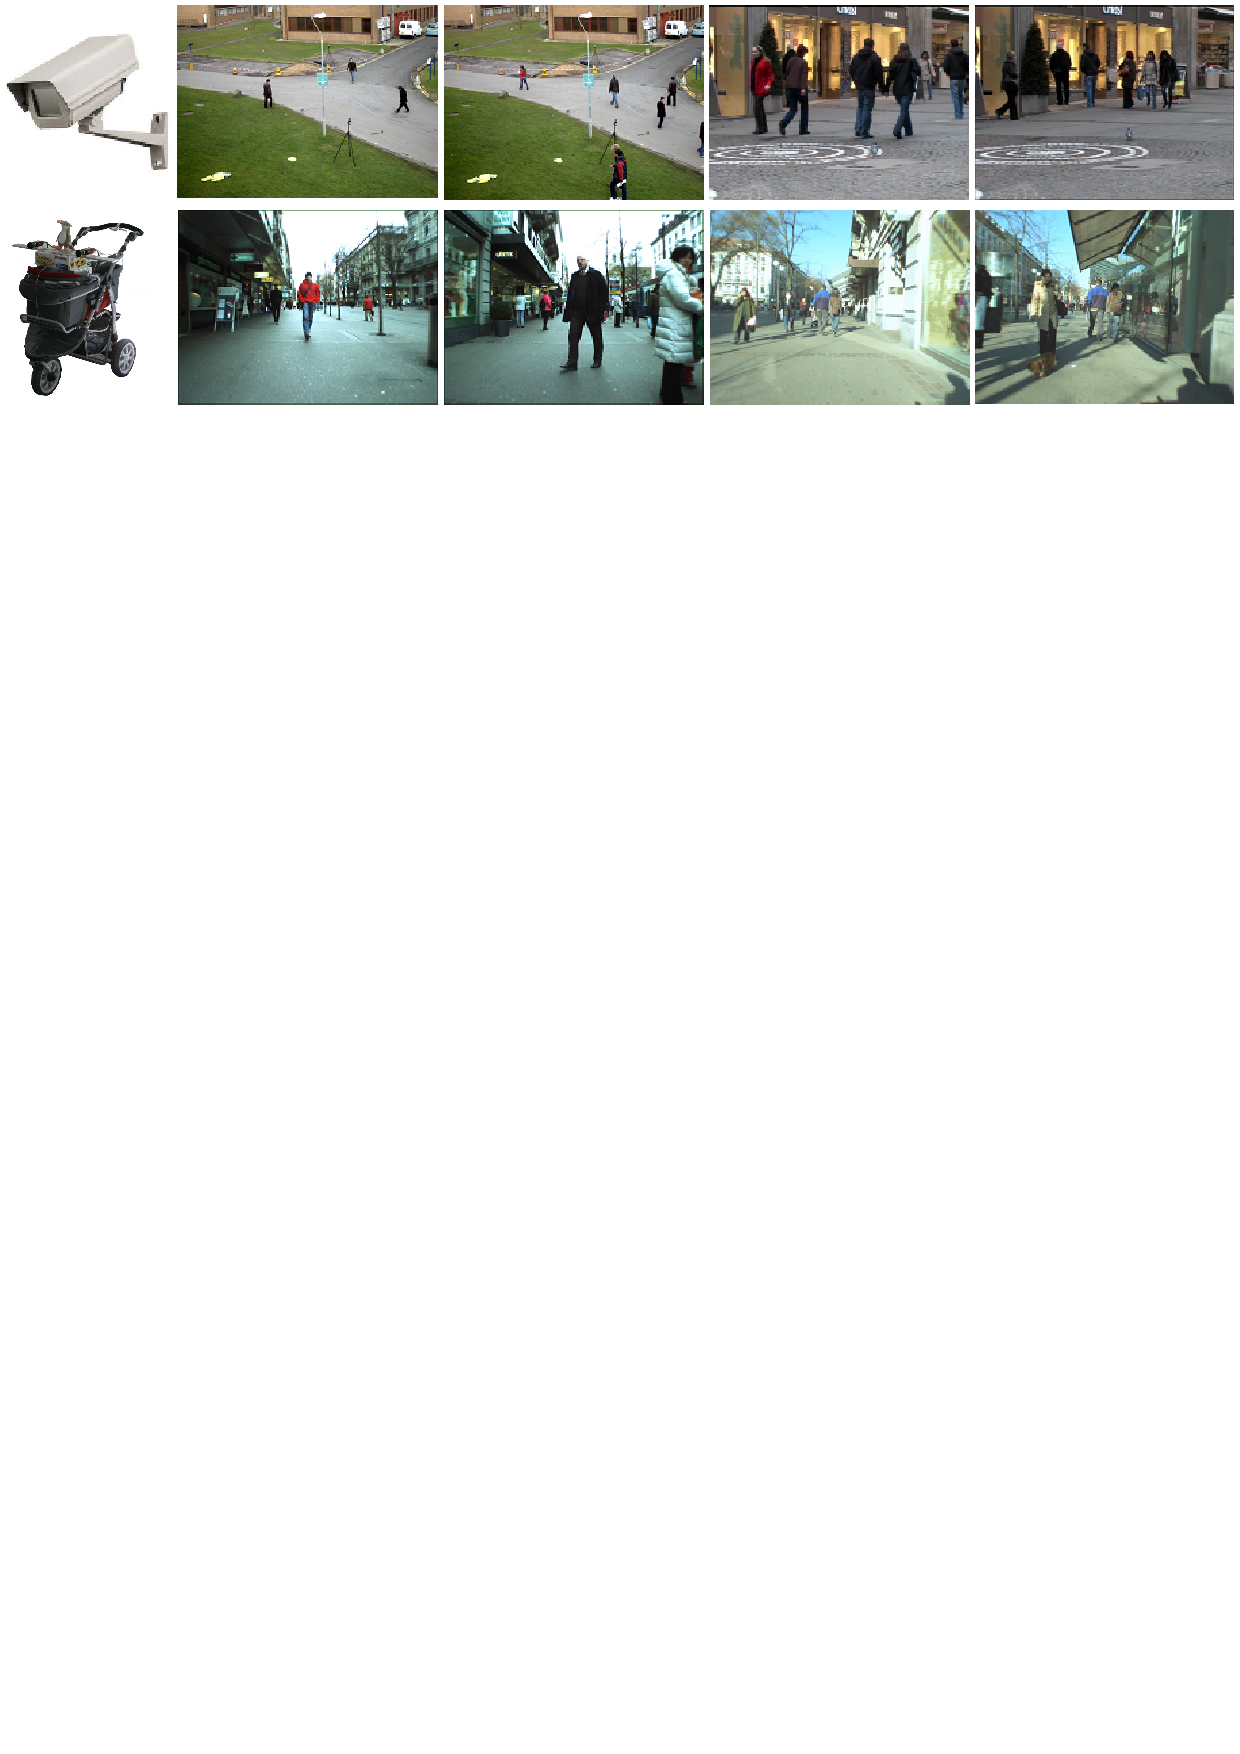
\includegraphics[width=0.95\textwidth]{scenes}
	\caption{图例}
	\label{fig:scenes}
\end{figure}

表例子。推荐使用这种三行表。缺省值使用三个“-”产生长横线“---”。

\begin{table}[!t]
\caption{示例表}
\label{tab:eg}
\vspace{0.5em}
\centering
\wuhao
	\begin{tabular}{ccccc}
	\toprule[1.5pt]
	表头 & 栏1 & 栏2 & 栏3 & 栏4 \\
	\midrule[1pt]
	内容1 & b & --- & $768 \times 576$ & 19 \\
	内容1 & a & 240/7 & $768 \times 576$ & --- \\
	\bottomrule[1.5pt]
	\end{tabular}
\end{table}

公式例子,与普通Latex数学公式无异。

\begin{equation}
1+1=2
\end{equation}


% !Mode:: "TeX:UTF-8"

\chapter{相关研究}

也有另一种结构将相关研究放在第一章,从第二章开始讲述自己的研究。

\section{第一节}

呵呵

\subsection{第一节的第一小节}

哈哈

\subsection{第一节的第二小节}

嘿嘿

\section{第二节}

aa

\subsection{第二节的第一小节}

bb


%%%%%%%%%%  参考文献  %%%%%%%%%%
\lhead{}
\rhead{}
\chead{\song\wuhao 中山大学硕士学位论文} % 覆盖设置页眉内容
\defaultfont
\bibliographystyle{references/TJUThesis}
\phantomsection
\markboth{参考文献}{参考文献}
\addcontentsline{toc}{chapter}{参考文献}       % 参考文献加入到中文目录
%\nocite{*}                                     % 若将此命令屏蔽掉,则未引用的文献不会出现在文后的参考文献中
\bibliography{references/thesis}

% ——————————————————————————————————————————————
% 以下是论文附录,在appendix子文件下

% 重新设置想要的chapter格式
\titleformat{\chapter}{\centering\sihao\hei}{\chaptername}{2em}{}

% 攻读硕士学位期间发表学术论文情况
% !Mode:: "TeX:UTF-8"

\markboth{攻读硕士学位期间发表学术论文情况}{攻读硕士学位期间发表学术论文情况}
\addcontentsline{toc}{chapter}{攻读硕士学位期间发表学术论文情况}
% 如果需要从该页开始从 1 开始编页,则取消以下注释
%\setcounter{page}{1}
\chapter*{攻读硕士学位期间发表学术论文情况}

\begin{enumerate}
	% 盲审时
	\item The paper title [J/C...]. Publish whereabout, 2014, 21(3): 288-291. (第一作者,导师为第一作者)(与学位论文第n章相关)(盲审时,不要出现名字)
	% 提交时
	\item Authors. The paper title [J/C...]. Publish whereabout, 2014, 21(3): 288-291. (提交时)
\end{enumerate}

% 不显示页码,则取消以下注释
%\thispagestyle{empty}


% 致谢
% !Mode:: "TeX:UTF-8"

\markboth{致\quad 谢}{致\quad 谢}
\addcontentsline{toc}{chapter}{致\quad 谢} % 添加到目录中
\chapter*{致\quad 谢}

谨此向我的导师张三教授致以衷心的感谢和崇高的敬意!本论文的工作是在张老师的悉心指导下完成的。在传授予我专业知识和宝贵经验的同时,张老师以其严谨的治学态度和精益求精的工作作风不断促进论文相关工作的进行,使我受益匪浅。
 
在攻读硕士的这三年里,导师和实验室的同学们不仅为我创造了优越的科研和学习环境,使我得以在计算机科学领域中自由翱翔,同时在思想上、人生态度和意志品质方面给予了谆谆教诲,这些教益必将激励着我在今后的人生道路上奋勇向前。特别感谢实验室的甲师兄、乙同学以及其他师弟师妹,他们不仅在学术上给了我许多指引和建议,而且在生活上予以帮助,从他们身上我学到了很多知识。

感谢王五老师及其实验室的同学在领域一、领域二方面的学习给予我的帮助。他们开创性的研究拓展了我的学术视野,无数次的争论和探讨使我的研究工作有了长足的进展。

由衷感谢我的室友A、B和C同学,以及其他经常到我们宿舍进行学习交流的D、E、F和G同学,是他们令我的学习生活都更加充满动力。
衷心的感谢我的父母和其他亲朋好友对我的关心、支持和理解,没有他们对我的关心、鼓励和支持,我无法完成现在的硕士学业。 

最后,感谢所有曾经教育和帮助过我的所有老师。衷心地感谢为评阅本论文而付出宝贵时间和辛勤劳动的专家和教授们!

% 如果需要加名字和日期(日期根据生成文档日期变更)
\maketime



\clearpage

% 结束中文字体使用
\end{CJK*}

% 结束全文
\end{document}